% IITG BSc (Hons) DS&AI Term Project Report
% Self-contained emulation of the course template (ICASSP-style, two-column).
% Compile with pdfLaTeX on Overleaf. Upload together with the three fig_*.png files.
\documentclass[a4paper,twocolumn,10pt]{article}

\usepackage[a4paper,top=2.2cm,bottom=2.2cm,left=1.9cm,right=1.9cm,columnsep=0.6cm]{geometry}
\usepackage{newtxtext,newtxmath}          % Times, as in the template
\usepackage{amsmath,amssymb}
\usepackage{graphicx}
\usepackage{dblfloatfix}      % lets full-width figures place on the current page, not drift to the end
\usepackage{booktabs}
\usepackage{xurl}   % break long URLs anywhere so DOIs/links wrap inside narrow columns
\usepackage{titlesec}
\usepackage[labelfont=bf,labelsep=period,font=small]{caption}
\usepackage[hidelinks]{hyperref}

% --- template-style section headings: "1. INTRODUCTION" centered bold caps ---
\titleformat{\section}{\centering\normalsize\bfseries}{\thesection.}{0.5em}{\MakeUppercase}
\titleformat{\subsection}{\normalsize\bfseries}{\thesubsection.}{0.5em}{}
\titlespacing{\section}{0pt}{10pt}{6pt}
\titlespacing{\subsection}{0pt}{8pt}{4pt}
\renewcommand{\figurename}{Fig.}

\begin{document}

% ------------------------------------------------------------------ title block
\twocolumn[{
\centering
{\large\bfseries CAN MACHINE-LEARNING AND DEEP-LEARNING MODELS FORECAST DAILY EQUITY VOLATILITY BETTER THAN CLASSICAL BASELINES?\par}
\vspace{4mm}
{\itshape François Schmitt (Roll Number: 23035010523)\par}
\vspace{4mm}
Term Project Report\\
Trimester 9\\
\vspace{3mm}
B.Sc.\ (Honours) Data Science and Artificial Intelligence\\
Indian Institute of Technology Guwahati, India\\
{\ttfamily f.schmitt@op.iitg.ac.in}\par
\vspace{7mm}
}]

% ------------------------------------------------------------------ abstract
\begin{center}\textbf{ABSTRACT}\end{center}
\noindent
This report presents a self-guided term project on one-day-ahead volatility forecasting for equity indices. Volatility drives option pricing, value-at-risk and position sizing, and, unlike the direction of returns, is strongly persistent and therefore forecastable. The objective was to test whether machine-learning (gradient-boosted trees) and deep-learning (LSTM) models can outperform well-implemented classical baselines. Eight models (naive, 21-day rolling variance, RiskMetrics EWMA, GARCH(1,1), GJR-GARCH, EGARCH, a walk-forward XGBoost and a regularized LSTM) were evaluated on 17 years of S\&P~500 daily returns (2008--2024) under a strict walk-forward protocol with no look-ahead bias, using the noise-robust QLIKE loss and the Diebold–Mariano test. A monthly re-estimated GARCH(1,1) achieved the best out-of-sample QLIKE (1.488), ahead of EGARCH, GJR-GARCH, EWMA, XGBoost and the LSTM; differences among the top three were statistically insignificant ($p=0.87$). XGBoost attained the lowest RMSE and MAE of all models, yet no learned model beat the GARCH family on the risk-relevant criterion. The project reproduces, with a fully reproducible open pipeline, the classic finding that GARCH is extremely hard to beat on daily data.

\vspace{2mm}
\noindent\textbf{\textit{Index Terms:}} Volatility forecasting, GARCH, QLIKE, XGBoost, LSTM, walk-forward evaluation

% ------------------------------------------------------------------ 1
\section{Introduction}

Volatility, the conditional standard deviation of an asset's returns, is the central quantity of financial risk management: it prices options, sets value-at-risk limits and margin requirements, and determines position sizes. Forecasting it accurately, even one day ahead, has direct practical value for any trading desk or risk function.

The problem is scientifically interesting because of a sharp asymmetry in predictability. The \emph{direction} of tomorrow's return is essentially unpredictable, but its \emph{magnitude} is not: calm days cluster with calm days and turbulent days with turbulent days. Classical econometrics has exploited this persistence for four decades, most famously through the GARCH family \cite{bollerslev1986}. In recent years, machine-learning and deep-learning models have been proposed as replacements, with mixed and sometimes contested results \cite{hansen2005}.

This project puts that proposition to a controlled test. Classical baselines and learned models were implemented within a single evaluation harness on 17 years of S\&P~500 daily data, with identical information sets, a shared out-of-sample window, a proxy-noise-robust loss and a formal significance test, so that any claimed improvement must survive statistical scrutiny rather than visual inspection.

Section~2 formulates the problem and lists the objectives. Section~3 details the methodology: the baselines, the learned models and the walk-forward protocol. Section~4 presents the experimental setup and results. Section~5 discusses and interprets the findings, Section~6 concludes, and Section~7 links the project artifacts.

% ------------------------------------------------------------------ 2
\section{Problem Statement and Objectives}

\subsection{Problem Statement}

Let $r_t = \ln(P_t/P_{t-1})$ be the daily log return of an asset, modelled as $r_t = \sigma_t z_t$ with $z_t$ zero-mean, unit-variance noise. The task is \textbf{one-day-ahead variance forecasting}: at the close of day $t-1$, output a forecast $\hat\sigma_t^2$ of day $t$'s conditional variance using information up to day $t-1$ only.

The fundamental difficulty is that true volatility is \emph{latent}: it is never observed on any day. Forecasts must be scored against a proxy; this project uses the squared return $r_t^2$, which is conditionally unbiased ($\mathbb{E}[r_t^2\,|\,\mathcal{F}_{t-1}]=\sigma_t^2$) but extremely noisy. The noise dictates two design constraints adopted throughout: (i) the headline evaluation loss must be robust to proxy noise, which motivates QLIKE \cite{patton2011}; and (ii) learned models cannot regress directly on $r_t^2$ without collapsing, which motivates a smoothed learning target (Section~3.2).

\begin{figure*}[!t]
\centering
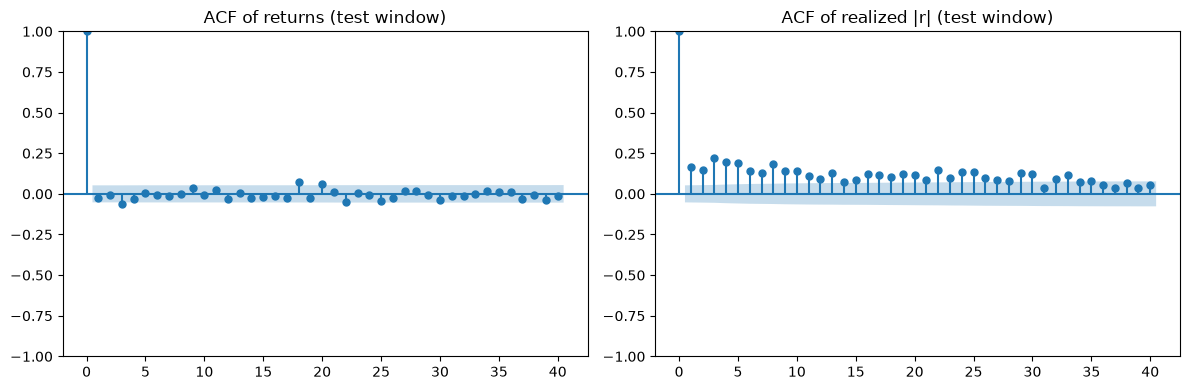
\includegraphics[width=\textwidth]{fig_correlogram.png}
\caption{Correlograms over the test window: ACF of returns (left) and of absolute returns (right), 40 lags with 95\% confidence bands. Returns are serially uncorrelated; absolute returns show slowly decaying, strongly significant autocorrelation, i.e.\ volatility clustering, the signal all models exploit.}
\label{fig:acf}
\end{figure*}

Figure~\ref{fig:acf} motivates the entire study: over the test window, the autocorrelation function of raw returns is flat (no linear predictability in the mean), while the ACF of absolute returns decays slowly and remains significant for dozens of lags. That persistence in magnitude is the only signal any model below exploits.

The scope is deliberately constrained: a single liquid index (S\&P~500), daily frequency, price-derived features only (no exogenous data), and a one-day horizon.

\subsection{Objectives}

\begin{enumerate}
  \item To implement honest classical baselines, namely naive, rolling, EWMA and the GARCH family (GARCH, GJR-GARCH, EGARCH) with periodic re-estimation, as the standard to beat.
  \item To design a leak-proof walk-forward evaluation harness with RMSE, MAE, QLIKE and the Diebold–Mariano test.
  \item To design and implement a walk-forward XGBoost forecaster with justified features and target.
  \item To design, implement and regularize an LSTM forecaster with explicit anti-leakage guards.
  \item To evaluate all models on a common out-of-sample window and determine whether observed differences are statistically significant.
  \item To deliver a reproducible, modular codebase.
\end{enumerate}

% ------------------------------------------------------------------ 3
\section{Methodology / Approach}

\subsection{Overall Workflow}

The pipeline runs end to end from raw prices to a significance-tested leaderboard: (1)~daily closes are downloaded and converted to log returns; (2)~the final 30\% of days is frozen once as the out-of-sample test window, shared by every model; (3)~each model produces one-day-ahead variance forecasts for the test window, using information up to the previous day only (classical models via recursions re-estimated periodically, learned models via walk-forward re-training); (4)~forecasts are scored against the squared-return proxy with RMSE, MAE and QLIKE; (5)~the best model is compared with the best remaining baseline by the Diebold–Mariano test. The five expensive model fits (three GARCH variants, XGBoost, LSTM) are mutually independent and run in parallel worker processes.

\subsection{Technical Details}

\textbf{Classical baselines.} The naive forecast is $\hat\sigma_t^2=r_{t-1}^2$; the rolling baseline is the variance of the previous 21 returns; EWMA is the RiskMetrics recursion $\hat\sigma_t^2=\lambda\hat\sigma_{t-1}^2+(1-\lambda)r_{t-1}^2$ with $\lambda=0.94$ \cite{riskmetrics1996}. The GARCH family models conditional variance as
\begin{equation}
\sigma_t^2 \;=\; \omega + \alpha\, r_{t-1}^2 + \beta\, \sigma_{t-1}^2 ,
\label{eq:garch}
\end{equation}
estimated by maximum likelihood (zero mean, normal innovations). GJR-GARCH \cite{glosten1993} adds the threshold term $\gamma\, r_{t-1}^2\,\mathbf{1}[r_{t-1}<0]$ to capture the leverage effect; EGARCH \cite{nelson1991} models $\ln\sigma_t^2$ with a signed standardized-residual term, guaranteeing positivity by construction. All three are re-estimated every 22 trading days on an expanding window; between refits the fitted recursion is rolled forward daily with observed returns. The hand-rolled recursions were verified against the reference implementation's internal source so that daily updates match the fitted parameters exactly.

\textbf{Features and target (shared by both learned models).} Features at row $t$ use data through $t-1$ only: lagged returns and squared returns (lags 1--10), realized variance over the past 5 and 21 days (spanning the multi-horizon structure of the HAR model \cite{corsi2009}), and the 5-day mean absolute return. Signed return lags let the models discover the leverage effect on their own. The learning target is
\begin{equation}
y_t \;=\; \ln\Big(\tfrac{1}{5}\textstyle\sum_{j=0}^{4} r_{t+j}^2 \;+\; \varepsilon\Big),
\label{eq:target}
\end{equation}
the log of forward 5-day average squared returns: averaging suppresses proxy noise and the log makes the target approximately Gaussian. Because $y_t$ is only observed at $t+4$, every training set excludes a 5-day buffer of the most recent rows.

\textbf{XGBoost.} A gradient-boosted ensemble (400 trees, depth 3, learning rate 0.03, row/column subsampling 0.8, a deliberately conservative low-variance configuration) is re-trained from scratch every 22 days on all fully realized targets, mirroring the GARCH refit cadence so the comparison is fair. Warm-starting refits from the previous booster was evaluated and rejected: it changes ensemble composition for negligible savings, sacrificing reproducibility.

\textbf{LSTM.} A single-layer LSTM (32 hidden units, linear head) reads the previous 20 days of standardized features and predicts $y_t$. Anti-leakage guards are explicit: sequences are labelled by their final row; standardization uses training-window statistics only; the early-stopping validation slice is carved from the \emph{end of the training window}, never from test. Training uses Adam on MSE in log-variance space, mini-batches of 64, up to 200 epochs with patience 15 and best-checkpoint restoration, and a fixed seed. The architecture is deliberately small: roughly 2{,}600 noisy training sequences cannot support a deep stack.

\textbf{Evaluation losses.} RMSE and MAE are computed on the volatility scale ($\sqrt{\text{variance}}$) for interpretability. The headline criterion is
\begin{equation}
\mathrm{QLIKE} \;=\; \frac{1}{T}\sum_{t}\Big(\frac{p_t}{v_t} - \ln\frac{p_t}{v_t} - 1\Big),
\label{eq:qlike}
\end{equation}
with proxy $p_t=r_t^2$ and forecast $v_t=\hat\sigma_t^2$: QLIKE rankings are robust to noise in an unbiased proxy \cite{patton2011}, and the loss penalizes under-prediction of variance more heavily than over-prediction, the asymmetry a risk manager wants. Loss differences are tested with the Diebold–Mariano statistic \cite{diebold1995} with the Harvey–Leybourne–Newbold small-sample correction \cite{harvey1997} on per-day QLIKE differentials.

% ------------------------------------------------------------------ 4
\section{Experiments and Results}

\subsection{Experimental Setup}

\textbf{Data.} S\&P~500 index (\texttt{\^{}GSPC}) daily closes, 2008-01-01 to 2024-12-31, from Yahoo Finance (auto-adjusted), yielding 4{,}277 daily log returns from 2008-01-03 to 2024-12-30. The sample spans the 2008 financial crisis, the 2018 ``volmageddon'', the COVID-2020 crash, the 2022 bear market and several calm regimes.

\textbf{Split.} The final 30\% of observations forms the out-of-sample test window: 2{,}993 training days (2008-01-03 to 2019-11-20) and 1{,}284 test days (2019-11-21 to 2024-12-30). The test window contains the COVID crash, so models are stress-tested out of sample.

\textbf{Environment.} Windows~11, CPU only; Python 3.13 with \texttt{numpy}~2.4.4, \texttt{pandas}~3.0.2, \texttt{arch}~8.0.0, \texttt{xgboost}~3.3.0, \texttt{torch}~2.12.1, \texttt{statsmodels}~0.14.6. All seeds fixed (42); one shared split; the full pipeline executes in about one minute with the five heavy fits in parallel processes.

\subsection{Results}

Table~\ref{tab:leaderboard} reports the leaderboard over the 1{,}284-day test window, sorted by QLIKE. The LSTM covers 1{,}275 of 1{,}284 days because its first prediction requires a full 20-day feature sequence. The naive baseline's QLIKE of $1.19\times10^{3}$ reflects a property of the loss, which diverges whenever a near-zero variance forecast meets a non-zero realization.

\begin{table}[t]
\centering
\caption{Out-of-sample leaderboard, test window 2019-11-21 to 2024-12-30 (1{,}284 days), sorted by QLIKE (lower is better). RMSE and MAE on the volatility scale; QLIKE on the variance scale. Best value per column in bold.}
\label{tab:leaderboard}
\small
\begin{tabular}{lrrrr}
\toprule
Model & $N$ & RMSE & MAE & QLIKE \\
\midrule
GARCH(1,1)      & 1284 & 0.00887 & 0.00633 & \textbf{1.4879} \\
EGARCH(1,1)     & 1284 & 0.00852 & 0.00603 & 1.4943 \\
GJR-GARCH(1,1)  & 1284 & 0.00881 & 0.00611 & 1.4974 \\
EWMA(0.94)      & 1284 & 0.00934 & 0.00657 & 1.5161 \\
XGBoost         & 1284 & \textbf{0.00816} & \textbf{0.00547} & 1.5567 \\
Rolling(21)     & 1284 & 0.00948 & 0.00646 & 1.5798 \\
LSTM            & 1275 & 0.00965 & 0.00570 & 1.5915 \\
Naive           & 1284 & 0.01114 & 0.00747 & 1192.69 \\
\bottomrule
\end{tabular}
\end{table}

\begin{figure*}[!t]
\centering
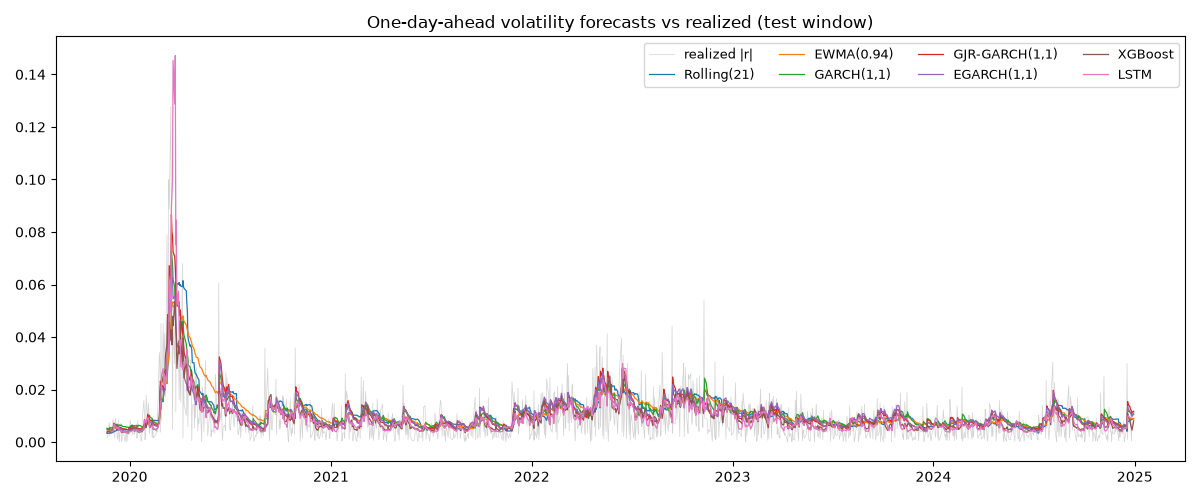
\includegraphics[width=\textwidth]{fig_forecasts_vs_realized.png}
\caption{One-day-ahead volatility forecasts of all models (naive omitted for legibility) against realized $|r_t|$ (grey), test window 2019-11-21 to 2024-12-30. All models track the same volatility clusters; they differ in smoothness and in responsiveness at eruptions such as COVID-2020.}
\label{fig:forecasts}
\end{figure*}

Figure~\ref{fig:forecasts} overlays every model's one-day-ahead volatility forecast on realized $|r_t|$ across the test window; Figure~\ref{fig:best} isolates the leaderboard winner against realized volatility. The Diebold–Mariano test between the two best models, GARCH(1,1) versus EGARCH(1,1) on per-day QLIKE, yields a statistic of $-0.166$ with $p=0.868$: the difference is not significant at any conventional level. The LSTM early-stopped at epoch 70 of a 200-epoch budget with best validation MSE (log-variance) of 0.642.

\begin{figure}[!t]
\centering
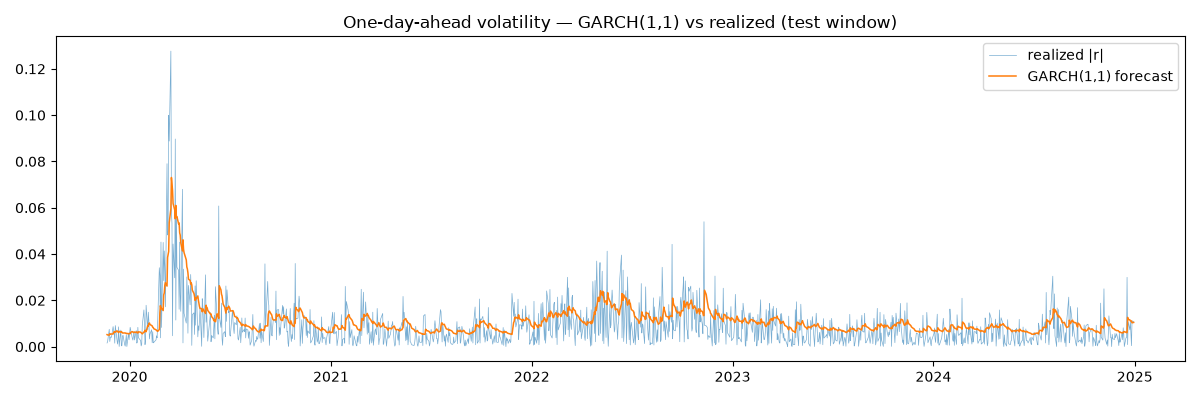
\includegraphics[width=\columnwidth]{fig_best_vs_realized.png}
\caption{Best model by QLIKE, GARCH(1,1), against realized volatility over the test window.}
\label{fig:best}
\end{figure}

% ------------------------------------------------------------------ 5
\section{Discussion}

\textbf{Why the GARCH family swept the QLIKE podium.} Four compounding reasons emerged. First, the exploitable signal in daily data is one-dimensional, namely persistence in return magnitude (Fig.~\ref{fig:acf}), and the GARCH recursion~\eqref{eq:garch} encodes exactly that shape with three parameters; the learned models must rediscover the recursion from finite noisy data before they can improve on it. Second, maximum likelihood estimates GARCH against the correct variance objective, whereas the learned models train on the smoothed surrogate~\eqref{eq:target}, which is necessary to avoid proxy-noise collapse but biases them toward smoothness. Third, roughly 3{,}000 noisy training observations is a small-data regime that favours 3-parameter models over 32-unit networks; reported deep-learning wins in this literature typically involve intraday realized-variance data, large cross-sections of assets or exogenous information. Fourth, QLIKE's asymmetry~\eqref{eq:qlike} rewards fast upward reactions: GARCH-type recursions respond to a single large return the next day, while tree ensembles and MSE-trained sequence models arrive late to eruptions and are charged heavily for it.

\textbf{Trade-offs observed.} XGBoost's best-in-class RMSE and MAE alongside a fifth-place QLIKE (Table~\ref{tab:leaderboard}) is the clearest trade-off: the smoothed target makes it accurate on average but slow at spikes, and the two metric families price those errors differently. Similarly, the leverage-effect models (EGARCH, GJR) improved point accuracy over plain GARCH but not QLIKE, and not significantly: the leverage effect is real but bought no significant one-day-ahead edge on this sample. Warm-starting XGBoost refits traded reproducibility for negligible speed and was rejected.

\textbf{Limitations.} (i)~Single asset and single test window: conclusions concern the S\&P~500 over 2019--2024, not ML-for-volatility in general. (ii)~The squared-return proxy is the noisiest admissible choice; intraday realized variance would sharpen both training and evaluation. (iii)~Hyperparameter search was deliberately modest, so the learned models' ceilings may be somewhat higher than reported, though the QLIKE gap ($\approx$0.07--0.10) makes a rank reversal unlikely. (iv)~Single seed per learned model. (v)~The DM test compares the two best models selected on the same test data, a mild selection bias; at $p=0.868$ this caveat is immaterial.

% ------------------------------------------------------------------ 6
\section{Conclusion and Future Work}

Under a leak-proof walk-forward protocol on 17 years of S\&P~500 data, a monthly re-estimated GARCH(1,1) delivered the best one-day-ahead variance forecasts by QLIKE, with EGARCH and GJR-GARCH statistically indistinguishable behind it, and no learned model outranked the GARCH family on the risk-relevant criterion. The answer to the project's question is a well-supported \emph{no}, with the nuance that the learned models were not poor (XGBoost won both symmetric metrics) but were beaten where it matters by a 40-year-old model with three parameters, consistent with \cite{hansen2005}.

The main learning outcomes were methodological: constructing a genuinely leak-free walk-forward harness (target buffering, train-only scaling, end-of-train validation) proved harder and more consequential than model building, and the choice of loss function changed the ranking of models, a reminder that ``better'' is undefined until the metric is.

Future work: realized-variance targets from intraday data (the HAR-RV setting \cite{corsi2009}), exogenous features such as the VIX term structure, multi-asset pooling to enlarge the effective training set, hybrid GARCH-plus-ML residual models, probabilistic forecasts under proper scoring rules, and robustness runs across assets (Nifty~50, gold, BTC) and across seeds.

% ------------------------------------------------------------------ 7
\section{Artifacts and Demonstrations}

\begin{itemize}
  \item \textbf{Code repository:} \url{https://github.com/iitgF/volatility-forecasting}. Contains the modular \texttt{volforecast} Python package (configuration, data, metrics, features, baselines, XGBoost, LSTM, evaluation, process-parallel pipeline) and both notebooks.
  \item \textbf{LaTeX source (Overleaf):} \url{https://www.overleaf.com/project/6a48e18e7dee3049b3ee4209}
  \item \textbf{Video demonstration:} \url{https://youtu.be/XXXXXXXXXXX} \emph{(placeholder, to be replaced with the final recording)}.
  \item \textbf{Consolidated notebook:} \texttt{volatility\_forecasting\_consolidated.ipynb}, the full study in a single annotated notebook, every module inline with a detailed introduction, executed end-to-end with all results and figures reproduced in this report.
  \item \textbf{Starter/development notebook:} \texttt{volatility\_forecasting\_starter.ipynb}, importing from \texttt{volforecast}.
\end{itemize}

% ------------------------------------------------------------------ 8
\newpage
\begin{thebibliography}{9}

\bibitem{bollerslev1986}
T.~Bollerslev, ``Generalized autoregressive conditional heteroskedasticity,'' \textit{Journal of Econometrics}, vol.~31, no.~3, pp. 307--327, 1986. \url{https://doi.org/10.1016/0304-4076(86)90063-1}

\bibitem{nelson1991}
D.~B. Nelson, ``Conditional heteroskedasticity in asset returns: A new approach,'' \textit{Econometrica}, vol.~59, no.~2, pp. 347--370, 1991. \url{https://doi.org/10.2307/2938260}

\bibitem{glosten1993}
L.~R. Glosten, R.~Jagannathan, and D.~E. Runkle, ``On the relation between the expected value and the volatility of the nominal excess return on stocks,'' \textit{Journal of Finance}, vol.~48, no.~5, pp. 1779--1801, 1993. \url{https://doi.org/10.1111/j.1540-6261.1993.tb05128.x}

\bibitem{diebold1995}
F.~X. Diebold and R.~S. Mariano, ``Comparing predictive accuracy,'' \textit{Journal of Business \& Economic Statistics}, vol.~13, no.~3, pp. 253--263, 1995. \url{https://doi.org/10.1080/07350015.1995.10524599}

\bibitem{riskmetrics1996}
J.P.~Morgan/Reuters, \textit{RiskMetrics: Technical Document}, 4th~ed., 1996.

\bibitem{harvey1997}
D.~Harvey, S.~Leybourne, and P.~Newbold, ``Testing the equality of prediction mean squared errors,'' \textit{International Journal of Forecasting}, vol.~13, no.~2, pp. 281--291, 1997. \url{https://doi.org/10.1016/S0169-2070(96)00719-4}

\bibitem{hansen2005}
P.~R. Hansen and A.~Lunde, ``A forecast comparison of volatility models: Does anything beat a GARCH(1,1)?'' \textit{Journal of Applied Econometrics}, vol.~20, no.~7, pp. 873--889, 2005. \url{https://doi.org/10.1002/jae.800}

\bibitem{corsi2009}
F.~Corsi, ``A simple approximate long-memory model of realized volatility,'' \textit{Journal of Financial Econometrics}, vol.~7, no.~2, pp. 174--196, 2009. \url{https://doi.org/10.1093/jjfinec/nbp001}

\bibitem{patton2011}
A.~J. Patton, ``Volatility forecast comparison using imperfect volatility proxies,'' \textit{Journal of Econometrics}, vol.~160, no.~1, pp. 246--256, 2011. \url{https://doi.org/10.1016/j.jeconom.2010.03.034}

\end{thebibliography}

\end{document}
